\documentclass[12pt,a4paper]{report}
\usepackage[utf8]{inputenc}
\usepackage[english]{babel}
\usepackage{amsmath}
\usepackage{amsfonts}
\usepackage{mathrsfs}
\usepackage{amsthm}
\usepackage{graphicx}
\usepackage{xcolor}
\usepackage[left=2cm,right=2cm,top=2cm,bottom=2cm]{geometry}

\usepackage{listings}

\usepackage{tikz}

\usepackage{cancel}

\renewcommand{\baselinestretch}{1.5} 

\lstnewenvironment{javacode}{%
\renewcommand\lstlistingname{Java Code}}{}

\lstset{
language=java,
basicstyle=\ttfamily,
frame=single,
backgroundcolor=\color{lightgray}
}

\theoremstyle{theorem}
\newtheorem{proposition}{Proposition}

\theoremstyle{definition}
\newtheorem{definition}{Definition}
\newtheorem{example}{Example}
\newtheorem{counterexample}{Counter-example}

\author{Justin Dekeyser}
\title{Introduction to Category Theory through Kleisli composition}
\begin{document}

\maketitle
\tableofcontents

\begin{abstract}
The purpose of this short document is to introduce
Category Theory through the specific context of Kleisli composition.
This perspective might be best suited for an audience of
programmers with a hands-on approach to monads, mainly through usages
and pragmatic use cases. Relying on well-known constructions in Java,
we introduce the idea of Category. We demonstrate how monads naturally
arise from this sole idea, without requiring the usual heavy material
that are natural transformations and adjunctions.

In order to make things are accessible as possible,
we have made the choice to keep the presentation agnostic of any
standard library. We use Java, for its ease of reading, its wide audience,
its static typing and the level of abstraction it allows.
\end{abstract}

\chapter{Review on functions}

\section{Methods and instructions}

Let us consider two methods in Java:

\renewcommand{\baselinestretch}{1} 
\selectfont
\begin{javacode}
static Double divideByTwo(Double x)
  { return x / 2.; }

static Double plusOne(Double x)
  { return x + 1.; }
\end{javacode}
\renewcommand{\baselinestretch}{1.5} 
\selectfont

Methods in Java are high level language constructions,
that represent code jumps in the byte-code. Might them be static
or instance-dependent, the methods (in Java, C, \ldots) are essentially
code jumps. Invoking a method
usually implies low-level interactions like:
\begin{enumerate}
	\item pushing the arguments of the method on the stack,
	\item jumping to the method's first line of code,
	\item letting the method load back arguments from the stack,
	\item performing the computation,
	\item pushing the result on the stack
	\item jumping back to the method invoke point,
	\item loading the result out of the stack.
\end{enumerate}
The accurate process might depend on the language and the computer.
Below is an illustration of that process, viewed through the Java Byte-code:

\pagebreak

\renewcommand{\baselinestretch}{1} 
\selectfont
\begin{javacode}
static divideByTwo(Ljava/lang/Double;)Ljava/lang/Double;
 L0
  LINENUMBER 8 L0
  ALOAD 0
  INVOKEVIRTUAL java/lang/Double.doubleValue ()D
  LDC 2.0
  DDIV
  INVOKESTATIC java/lang/Double.valueOf (D)Ljava/lang/Double;
  ARETURN
static plusOne(Ljava/lang/Double;)Ljava/lang/Double;
 L0
  LINENUMBER 12 L0
  ALOAD 0
  INVOKEVIRTUAL java/lang/Double.doubleValue ()D
  DCONST_1
  DADD
  INVOKESTATIC java/lang/Double.valueOf (D)Ljava/lang/Double;
  ARETURN
\end{javacode}
\renewcommand{\baselinestretch}{1.5} 
\selectfont

Similarly to most languages, methods in Java cannot be
composed to obtain new methods. As an example, we observe that
an instruction of the kind

\renewcommand{\baselinestretch}{1} 
\selectfont
\begin{javacode}
divideByTwo(plusOne(x));
\end{javacode}
\renewcommand{\baselinestretch}{1.5} 
\selectfont

would yield the byte-code instructions

\renewcommand{\baselinestretch}{1} 
\selectfont
\begin{javacode}
INVOKESTATIC Play.plusOne (Ljava/lang/Double;)Ljava/lang/Double;
INVOKESTATIC Play.divideByTwo (Ljava/lang/Double;)Ljava/lang/Double;
\end{javacode}
\renewcommand{\baselinestretch}{1.5} 
\selectfont

which shows that there was no third method created by the composition
of the previous ones. In fact, chaining method invocations directly
translates as chaining low-level instructions.

\section{Functions and objects}

In most languages, especially in dynamic languages like Python and JavaScript
for example, methods are also objects. This approach can be followed
in Java too, up to defining an abstraction that encodes the
method signature\footnote{The Java Standard Library 
comes with a built-in notion of function,
namely \lstinline{java.util.function.Function}{},
but we have chosen to re-define this type in this text.}:

\renewcommand{\baselinestretch}{1} 
\selectfont
\begin{javacode}
@FunctionalInterface
interface Function<InputType, OutputType>
{
  OutputType apply(InputType input);
}
\end{javacode}

\renewcommand{\baselinestretch}{1.5} 
\selectfont

The following piece of code demonstrates how to instantiate functions
out of methods, by a language construction referred to as
\emph{method reference}:

\renewcommand{\baselinestretch}{1} 
\selectfont

\begin{javacode}{From methods to functions}
Function<Double, Double> divideByTwo = DemoClass::divideByTwo;
Function<Double, Double> plusOne = DemoClass::plusOne;
\end{javacode}

\renewcommand{\baselinestretch}{1.5} 
\selectfont

Compared to methods, \emph{function composition} is possible,
as long as the function objects know how to compose themselves.
Consider for example the following compose:

\renewcommand{\baselinestretch}{1} 
\selectfont
\begin{javacode}
static <X, Y, Z> Function<X, Z> compose(
  Function<Y, Z> g,
  Function<X, Y> f
)
  { return x -> g.apply(f.apply(x)); }
\end{javacode}

\renewcommand{\baselinestretch}{1.5} 
\selectfont

In the above code, we have used a lambda-expression syntax, to define and
instantiate a new object of type \lstinline{Function}{}.
As an example, we can indeed compose function-objects and create new ones:

\renewcommand{\baselinestretch}{1} 
\selectfont
\begin{javacode}
Function<Double, Double> divideByTwo = DemoClass::divideByTwo;
Function<Double, Double> plusOne = DemoClass::plusOne;

Function<Double, Double> plusOneThenDivideByTwo
	= compose(divideByTwo, plusOne);
\end{javacode}

\renewcommand{\baselinestretch}{1.5} 
\selectfont

If we were to write function composition
with mathematical symbols, we usually would write:
	\[ (g\circ f)(x) = g(f(x)) .\]
In is interesting to note here, that we somehow find back the two
approaches that exist in programming. The left-hand side 
is the invoke of one function, namely $(g\circ f)$.
The right-hand side however, defines an algorithm to evaluate $(g\circ f)$
on a point:
first apply $f$ on $x$, and then apply $g$ on the result $f(x)$.
It is important to note that this expansion, as a definition, is always correct;
while it might not be interesting to apply in practice.
For example, considering
	\[ \big((\cdot)^{\frac{1}{3}} \circ (\cdot)^3\big)(x) = x ,\]
we see that we do not have to apply to function
in order to evaluate $\big((\cdot)^{\frac{1}{3}} \circ (\cdot)^3\big)$,
as this function turns out to be the identity. Algorithms might therefore
be modified depending on their context. This is what we would do, in
Object Oriented style:

\renewcommand{\baselinestretch}{1} 
\selectfont
\begin{javacode}
default <MiddleType> Function<InputType, MiddleType> then(
  Function<OutputType, MiddleType> g
)
  { return compose(g, this); }
\end{javacode}

\renewcommand{\baselinestretch}{1.5} 
\selectfont

Composing can now be phrased in the context of one of the member,
for example:

\renewcommand{\baselinestretch}{1} 
\selectfont
\begin{javacode}
Function<Double, Double> divideByTwo = DemoClass::divideByTwo;
Function<Double, Double> plusOne = DemoClass::plusOne;

Function<Double, Double> plusOneThenDivideByTwo
	= plusOne.then(divideByTwo);
\end{javacode}

\renewcommand{\baselinestretch}{1.5} 
\selectfont

The Object Oriented style has the benefit of making it explicit that
the function \lstinline{plusOne}{} actually owns the composition
algorithm, and might override the default implementation,
or define overloads. Consider the following example, which takes benefit
of overloading to mitigate stack-overflows:

\renewcommand{\baselinestretch}{1} 
\selectfont
\begin{javacode}
@FunctionalInterface
interface DoubleFunction extends Function<Double, Double>
{
  
  default DoubleFunction then(DoubleFunction g)
  {
    record BackedByList(DoubleFunction[] stack) {
      @Override
      public DoubleFunction then(DoubleFunction z)
      {
        var newStack = new DoubleFunction[stack.length + 1];
        arraycopy(stack, 0, newStack, 0, stack.length);
        newStack[stack.length] = z;
        return new BackedByList(newStack);
      }
      
      @Override
      public Double apply(Double x)
      {
        for(var f: stack)
          x = f.apply(x);
        return x;
      }
    }
    return new BackedByList(new DoubleFunction[]{this, g});
  }
}
\end{javacode}

\renewcommand{\baselinestretch}{1.5} 
\selectfont

This extension takes benefit of object oriented style, to
override the behavior of \lstinline{then}{} and store factors of a composition
in an (effectively) immutable array. Note that the record type is
unreachable from the outside, which prevents accidental mutation of
array elements. With this implementation, composing a very large number of
functions can be done without throwing stack-overflow exceptions.

\section{Functions are nearly monoids}

Since the algorithm that describes function composition, often turns out
to be an
implementation detail, it is relevant to look for \emph{properties}
the composition enjoys and that would allow us to reason about it.

\paragraph*{Neutral element}
There is a special function, that acts as nothing for composition.
This function is referred to as \emph{the identity function},
which we are going to denote ${\rm id}$:
	\[ f\circ {\rm id} = f = {\rm id} \circ f ,\]
or in other words: composing with the identity on the left or on the
right, has no effect.\footnote{Note that actually,
there is an infinite number of identities, as
they are all dependent on their domain. We should actually write
${\rm id}_X$ for the identity on the domain $X$, although we are going to
omit the subscript very often, for obvious clarity reasons.
We will come back on that later on.}

A descriptive implementation of the identity in mathematical symbols could be
	\[ {\rm id}(x) = x ,\]
while a Java implementation of the identity function, could be:

\renewcommand{\baselinestretch}{1} 
\selectfont

\begin{javacode}
static <X> Function<X, X> identity()
  { return x -> x; }
\end{javacode}

\renewcommand{\baselinestretch}{1.5} 
\selectfont

One should however observe, that the above implementation
is an implementation detail. As shown above, there might be many
functionally equivalent ways to write the identity function.
However, we can talk about \emph{the} identity as
the unique function that satisfy the axiom
	\[ f\circ {\rm id} = f = {\rm id} \circ f ,
		\quad \textrm{for any}\ f .\]
It is also important to realize
that the Java version cannot encode the above axiom,
but can only see it de facto realized. In other words: the fact that the
\lstinline{identity}{} method indeed returns an object that stands for the
identity of function, is a meta-information only available through
specification.

It is a general rule,
that {\bf most of the axioms} that are actually {\bf of fundamental importance},
sadly {\bf escape the type system}. General purpose programming languages
are not design to encode axioms.

\paragraph*{Associativity of composition}

Another important property of function composition is what we call
\emph{associativity}, and can be formulated through the formula
	\[ h\circ(g\circ f) = (h\circ g)\circ f ,\]
whenever it makes sense; that is: whenever the functions can indeed
be composed together.
That property is also the one that allows you to speak about
	\[ h\circ g\circ f, \]
without having to define a tri-operator $\circ$: it is implicitly understood that
	\[ h\circ g\circ f = h\circ(g\circ f) = (h\circ g)\circ f .\]
	
This is again a property that will
escape the type system.
In Java, associativity would yield to the functional equivalence
between \lstinline{compose(compose(h, g), f)}{}
and \lstinline{compose(h, compose(g,f))}{}.
One will obviously keep in mind, that this is \emph{not} an equality of
object references, but only an equality of behaviors: both
objects are \lstinline{Function}{} (of the same types) and their result
on the same argument is equivalent. (Note that we never defined a
\lstinline{equals}{} notion on the \lstinline{Function}{} type.)\footnote{The
pragmatic programmer would, for instance, encode the identity and associativity
axioms, via \emph{unit tests}. Unit tests play the role as a statistical way
of validating a rule: if the tests suite sampled a sufficiently fair
amount of use cases (and if all tests pass), then it it likely to properties
are valid. The process of sampling correctly the space of use cases,
is where the next struggle lies\ldots\ but
 this is out of the scope of the current
document.}

\paragraph*{Monoids}
The word \emph{monoid} refers to an algebraic structure that enjoys
an associative operation, for which there exists a neutral element.
We introduce the definition in a state-of-the-art style:

\begin{definition}
A monoid is a set $\mathcal{M}$ equipped with a bi-function
	\[ + : \mathcal{M}\times \mathcal{M} \to \mathcal{M} ,\]
and a special element called \emph{neutral element} $0\in\mathcal{M}$,
such that
	\begin{description}
		\item[Neutrality] For all element $m$ of the monoid $\mathcal{M}$,
		we have
			\[ m + 0 = m = 0 + m ,\]
		\item[Associativity] For all elements $m_1,m_2,m_3$ of the monoid
		$\mathcal{M}$, we have
			\[ m_1 + (m_2 + m_3) = (m_1 + m_2) + m_3 .\]
	\end{description}
\end{definition}
In the definition above, we have chosen the additive convention $(+,0)$
to refer to the monoid summation, and its neutral element. There are different
conventions possible, like the multiplicative one $(*,1)$.
In any case, the reader should keep in mind that \emph{we do not mean}
numeric operations here: the definition is more general and the examples
below demonstrate the structure on a standard pool of examples:
\begin{example}
The collection of natural numbers $\mathbb{N}$, equipped with the standard
addition $+$ and $0$ as neutral element, is a monoid.
\end{example}
\begin{example}
The collection of vectors in $N$-dimensions, with the standard addition of
vectors and the null vector as neutral element, is a monoid.
\end{example}
\begin{example}
The collection of non null integers $\mathbb{N}$, equipped with the standard
multiplication $*$ and $1$ as neutral element, is a monoid.
\end{example}
\begin{example}
Composition of linear applications from $\mathbb{R}^n$ to $\mathbb{R}^n$,
with the identity matrix as neutral element, is a monoid.
\end{example}
\begin{example}
The collection of words over an alphabet, equipped with the standard
concatenation and the empty word as neutral element, is a monoid.\footnote{In
Java and other languages, it is common to concatenate strings with a $+$
symbol. This can be misleading, as compared to the addition of numbers, the
concatenation of strings is a monoid operation but doesn't have inverse
(minus $-$), and is not commutative neither (the order matters). PHP has chosen
a dot operator $.$ to phrase the string concatenation: maybe not a bad idea
after all.}
\end{example}
\begin{counterexample}
The collection of real positive numbers, with the division, is not a monoid.
It has $1$ as neutral element, but it lacks associativity:
	\[ 2 / (3/4) = \frac{8}{3} \neq \frac{1}{6} = (2/3) / 4 .\]
\end{counterexample}
\begin{example}
The collection of functions from $X$ to $X$, with the composition
$\circ$ of function and the identity over $X$ as neutral,
is a monoid.
\end{example}

But the {\bf collection of all functions}, for the function composition,
{\bf is not a monoid}. Indeed, the composition of functions is actually
ill-defined on the entire collection: we cannot compose every function
together.

As an example, we can consider the subtype
\lstinline{DoubleFunction}{}, which corresponds to function from
\lstinline{Double}{} to themselves. This subset of functions is a valid
monoid, and as we have seen, we can equip this set with an associative
(and variadic) composition law. Such operation on the class of
\lstinline{Function}{} in general wouldn't be possible
without also weakening the types for the domains and the images.

\chapter{Category Theory}

In the previous chapter, we have discovered that there is a profound
typing issue while working with functions composable units.
Mathematically speaking, functions across different domains,
actually do not really fit the definition of monoids.

\section{Towards a functional framework}

In order to acquire a formalism to talk about functions in all their
generality, let's consider the following illustrations of functions:

\begin{center}
\begin{tikzpicture}
\filldraw[black] (0,0) circle (0.1);
\filldraw[black] (1,1) circle (0.1);
\filldraw[black] (.5,2) circle (0.1);
\draw {(0.5,1) ellipse (1 and 2)};

\filldraw[black] (10,1) circle (0.1);
\filldraw[black] (11,2) circle (0.1);
\filldraw[black] (10.5,0) circle (0.1);
\draw {(10.5,1) ellipse (1 and 2)};

\node at (0.5, -2)  {$X$};
\node at (10.5, -2) {$Y$};

\node at (2.5, 1) (X) {};
\node at (8.5, 1) (Y) {};
\node at (5.5, 1) {$f$};

\draw[->,>=stealth] (X.north) to [out=30,in=150] (Y.north);
\end{tikzpicture}
\end{center}
This is a schematic representation of a function, that maps points
from a set (or type) $X$, to points of a set (or type) $Y$.
Let's take some steps back, literally:
\begin{center}
\begin{tikzpicture}
\node at (2.5, 0) (X) {};
\node at (8.5, 0) (Y) {};
\node at (5.5, 0.5) {$f$};

\draw (X) circle (0.3);
\draw (Y) circle (0.3);

\node at (2.5, -1)  {$X$};
\node at (8.5, -1) {$Y$};

\draw[->,>=stealth] (3.5, 0) to (7.5, 0);
\end{tikzpicture}
\end{center}
Once we abstract away the elements and their mapping (that is to say:
the function implementation), a function 
actually looks more like an arrow that connects two
types, represented by nodes.
This is \emph{exactly} what Category Theory is all about.

\subsection{Objects and \cancel{functions} \cancel{arrows} morphisms}

A \emph{category} $\mathcal{C}$
is made of \emph{objects}, in the widest sense.
The collection of objects of a category are denoted by
${\rm Obj}(\mathcal{C})$. Usually, the collection of objects do not form
a set, in the set theoretic sense; hence we should not be allowed to
write $X\in{\rm Obj}(\mathcal{C})$
to phrase that $X$ is an object in the category
$\mathcal{C}$. Since we still want a notation for that, \emph{in this text},
we are going to use the type theoretic notation:
	\[ X : {\rm Obj}(\mathcal{C}) . \]
A category $\mathcal{C}$ is also composed of \emph{arrows},
or \emph{morphisms}, between those
objects. Given two objects $X$ and $Y$ from a category $\mathcal{C}$,
the collection of arrows between them is traditionally denoted by
${\rm Hom}(X,Y)$. Again, we are going to
shorten it by writing
	\[ f: {\rm Hom}(X,Y) ,\]
or often simply
	\[ f : X\to Y .\]
It has to be emphasized that \emph{morphisms are no functions}, but a more
general concept that is closer to edges in a graph.

\begin{example}
Since we are mainly interested in programming in Java,
we reserve the symbol
$\mathcal{F}$ to talk about the category of functions,
whose objects are types (in the Java sense) and the arrows
are instances of \lstinline{Function}{}. 
This does not mean functions are
functions of types, as one can find in languages like Zigg.
Functions map points $x$ of a given type $X$,
onto points $y$ of another type $Y$;
and that mapping induces a morphism $X\to Y$.
Morphisms in $\mathcal{F}$
are total functions (and never partial), and cannot throw errors.\footnote{In
other words, \emph{in this text}, we disallow ourselves to speak about functions
that throw errors (checked or unchecked), and function that return nothing
(\lstinline{void}{}) or a \lstinline{null}{} reference. \emph{But methods
can do it!}}
\end{example}

\pagebreak

\subsection{Formal definition}

So far, categories look like graphs where nodes are called objects,
and edges are called morphisms. Unlike graphs, categories
must obey some rules that translate morphism composition.

\begin{definition}
A Category $\mathcal{C}$ is the given of a collection of entities called
\emph{objects}, denoted ${\rm Obj}(\mathcal{C})$, together with a collection
of \emph{morphisms} ${\rm Hom}_{\mathcal{C}}(X,Y)$
from objects $X$ to $Y$, such that the
following conditions hold:
	\begin{description}
		\item[Composition] For all objects $X,Y,Z$ in ${\rm Obj}(\mathcal{C})$,
		and for any morphisms $f:X\to Y$ and $g:Y\to Z$, there exists a
		morphism
			\[ g\circ f : X\to Z \]
		from $X$ to $Z$;

\begin{center}
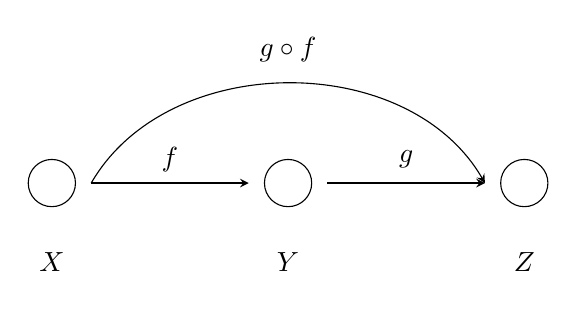
\begin{tikzpicture}
\node at (2.5, 0) (X) {};
\node at (5.5, 0) (Y) {};
\node at (8.5, 0) (Z) {};
\node at (4, 0.3) {$f$};
\node at (7, 0.3) {$g$};
\node at (5.5, 1.7) {$g\circ f$};

\draw (X) circle (0.3);
\draw (Y) circle (0.3);
\draw (Z) circle (0.3);

\node at (2.5, -1)  {$X$};
\node at (5.5, -1) {$Y$};
\node at (8.5, -1) {$Z$};

\draw[->,>=stealth] (3, 0) to (5, 0);
\draw[->,>=stealth] (6, 0) to (8, 0);
\draw[->,>=stealth] (3, 0) to [out=60,in=120] (8, 0);
\end{tikzpicture}
\end{center}
		\item[Neutral element] For all object $X$ in ${\rm Obj}(\mathcal{C})$,
		there exists a morphism
			\[ {\rm id}_X : X\to X;\]
		and for any morphism $f:X\to Y$ we have
			\[ f\circ {\rm id}_X = f = {\rm id}_Y \circ f ;\]
		\item[Associativity] For all objects $X,Y,Z,W$ in ${\rm Obj}(\mathcal{C})$
		and for all morphisms $f:X\to Y$, $g:Y\to Z$, $h:Z\to W$,
		we have
			\[ h\circ (g\circ f) = (h\circ g)\circ f .\]
	\end{description}
\end{definition}

\section{More than functions}

Most programs are not
only sequences of pure instructions:
in practice, programmers have a lot of contingent issues that happen
at runtime, or that depict hardware related concerns.

Below us a non-exhaustive list of situation where runtime, hardware,
or third-party libraries, would disallow you
to play within the bounds of scholar examples.

\subsection{IRL: There might be nothing to answer}
Imagine the following methods:

\renewcommand{\baselinestretch}{1} 
\selectfont
\begin{javacode}{Unfaithful data representation}
Integer opposite(Integer a)
  { return -a; }
  
Double toDouble(Long a)
  { return (double) a.longValue(); }
\end{javacode}

\renewcommand{\baselinestretch}{1.5} 
\selectfont

Although they seem fine, those methods might have undesirable behaviours.
The problems come from representation formats, inherent to the
realm of number representations on a finite number of bits.
The types \lstinline{Integer}{}, \lstinline{Long}{}
and \lstinline{Double}{}, actually do not stand for numbers, but for
representations of them. However, any sane programmer would \emph{think of them}
as being numbers, yielding to weird behaviours that are easily forgotten.

The following version of the same methods, might better phrase
the effective expectations about the results:

\renewcommand{\baselinestretch}{1} 
\selectfont

\begin{javacode}{Unfaithful data representation}
OptionalInt opposite(Integer a)
{
  return (a > Integer.MIN_VALUE)
           ? of(-a)
           : empty();
}
OptionalDouble toDouble(Long a)
{
  var doubleValue = (double) a.longValue();
  return ((long)doubleValue == a)
           ? of(doubleValue)
           : empty();
}
\end{javacode}

\renewcommand{\baselinestretch}{1.5} 
\selectfont

Another family of example, are programs that must be stopped
because they run into an infinite loop situation.
This is the case for algorithms that approximate solutions to
problems, like Newton-Rhapson method, for example.

\subsection{IRL: Hardware might break}
Another big kind of things that can badly happen at runtime,
is the presence of errors related to hardware.
The following example is a well-known way to compute the Fibonacci numbers,
that can throw an error:

\renewcommand{\baselinestretch}{1} 
\selectfont

\begin{javacode}{Hardware related issue}
Long fibonacci(Integer index)
{
  if(index <= 1) return 1L;
  else
    return fibonacci(index - 1) + fibonacci(index - 2);
}
\end{javacode}

\renewcommand{\baselinestretch}{1.5} 
\selectfont

It is obvious that this code is type-safe and functionally correct,
yet is will likely crash with a \lstinline{StackOverflowException}{}
as soon as the input becomes too large. The problem is that the runtime
has a hardware limit, and that limit cannot be foreseen easily.

When the compiler or runtime implements tail-recursion optimization,
it can detect those cases and refuse to compile if the recursive
call cannot be made tail-recursive; then only optimize
to prevent stack-size limit issues. But it is not often the case we
have tail-recursion optimization available.

\subsection{IRL: External resource connections might fail}

Input/Output operations are also a great source of errors.
Again, Java usually workarounds them by declaring a checked
\lstinline{IOException}{}, which makes it looks like an union type
between the expectation and the possible errors.

Cause of IO exceptions might not always be as predictable as
an absence of file on the disk, or a permission issue. It could also
occur during the process of a reading or writing, for example.

\subsection{IRL: The result might not be there yet}

It is often the case in concurrent programming that the result must be
delayed. Taking back the Fibonacci computer above,
we could for example decide to implement it as

\renewcommand{\baselinestretch}{1} 
\selectfont

\begin{javacode}{Future results}
Long fibonacci(Integer index)
{
  Long[] stack = {1L, 1L};
  while(index > 1) {
    Long next = stack[0] + stack[1];
    stack[0] = stack[1];
    stack[1] = next;
    index -= 1;
  }
  return stack[1];
}
\end{javacode}

\renewcommand{\baselinestretch}{1.5} 
\selectfont

but quickly rely on a concurrent solution:

\renewcommand{\baselinestretch}{1} 
\selectfont

\begin{javacode}{Future results}
FutureTask<Long> fibonacci(Integer index)
{
  Function<Integer, Long> engine = i -> {
    Long previous = 1L;
    Long result = 1L;
    while(i > 1) {
      Long next = result + previous;
      previous = result;
      result = next;
      i -= 1;
    }
    return result;
  };
  return new FutureTask<>(() -> engine(index));
}
\end{javacode}

\renewcommand{\baselinestretch}{1.5} 
\selectfont

The advantage is that not only the task could be called
immediately, but it could also be sent on an executor service
for parallel evaluation. The result occurs later, but not now.

\subsection{IRL: There might be many results}

Something that is less often the case, but still
valuable to think about, are the cases where functions would return
multiple values of the same type.

This could happen, for example, when the applied operation has
an uncertainty that disallows it to resolve with a single value.
For example:

\renewcommand{\baselinestretch}{1} 
\selectfont

\begin{javacode}{Multi results}
Double[] squareRoot(Double x)
{
  if(Double.isFinite(x))
    return new Double[]{
      -sqrt(abs(x)),
      sqrt(abs(x))
    };
  else if(Double.isNaN(x))
    return new Double[]{ Double.NaN };
  else
    return new Double[] {
      NEGATIVE_INFINITY,
      POSITIVE_INFINITY
    };
}
\end{javacode}

\renewcommand{\baselinestretch}{1.5} 
\selectfont

It is also the case where you expect multiple results out of a
database query, for example. Even when you query a database with
a given value of unique primary key, stricto senso, the SQL engine
returns a result set from where you usually pick only the first element,
yet the result is a potential plural.

\subsection{Should we panic?}

In an ideal world, most jobs can be achieved by considering a pure
mapping
	\[ f: X\to Y .\]
For different reasons, the return type would be modified in Java
to express realities from programs.

Forcefully, there is an application $\mathcal{M}$,
from ${\rm Obj}(\mathcal{C})$ to ${\rm Obj}(\mathcal{C})$,
that depicts the function with better accuracy:
	\[ \mathfrak{f} : X\to \mathcal{M}(Y) .\]

The problem of the operator $\mathcal{M}$ is that it breaks
our notion of composition, even in the categorical sense.
Within the category of functions,
an arrow
	\[ \mathfrak{f} : X\to \mathcal{M}(Y)\]
cannot be composed with an arrow
	\[ \mathfrak{g} : Y\to \mathcal{M}(Z) \]
in all generality: the range of $\mathfrak{f}$ does not agree at
all with the range of $\mathfrak{g}$.

There are two strategies:
	\begin{description}
		\item[Recovering as soon as possible]This is often the safest to
		do. It is actually equivalent to drawing an arrow
			\[ \mathcal{M}(Y) \to Y \]
		that pops out the initial value, or else recover with another one.
		In practice, this is the easiest way to get rid of issues, but
		it is not always possible to do so.
		\item[Seeking for an extension]Instead of viewing the range 
		as a problem, we could try to extend domains instead, and thus
		lifting morphisms from
			\[ Y\to \mathcal{M}(Z) \]
		to
			\[ \mathcal{M}(Y) \to \mathcal{M}(Z) .\]
	\end{description}

~\newline

\begin{center}
The latter is \emph{exactly} what Kleisli categories\footnote{and actually
monads} are all about!
\end{center}

\chapter{Kleisli Category}

In the previous chapter, we have seen that Category Theory is a framework
that fits really well the idea of function composition.
However, we also made a point that in practice, real world programming
does not deal with functions, but with functions that can suffer a bit
from runtime, for good or bad reasons.
In this chapter, we investigate further a prototype example
of such decoration, aside from any cultural choice made by programming
languages like Java. We then discover the notion of Kleisli Category.

\section{A lazy example}

The title is barely a word distortion.
We are going to focus on a special kind of
objects, that are lazy.
Laziness in programming, refers to the idea that things are computed
or evaluated, only when required. It is often the case we talk about
lazy functions but here, we are going to work on lazy objects.

We define a \emph{lazy object} as an object implementing the following
specification:

\renewcommand{\baselinestretch}{1} 
\selectfont

\begin{javacode}{Lazy object specification}
interface LazyObject<ObjectType>
{
  ObjectType get();
}
\end{javacode}

\renewcommand{\baselinestretch}{1.5} 
\selectfont

Lazy objects of type $X$ (which we right $\mathcal{L}(X)$ in
mathematical symbols) are therefore objects that one can get on-demand,
but won't be computed until really required. It is implicit in the above
specification, that we ask for the object to be always the same
(otherwise it would look more like a randomization process, than a lazy one).

Our goal is to show that lazy objects will induce a special way of composing
arrows, and we are going to use that prototype example to motivate
the notion of Kleisli category.

\subsection{The arrow signature}

As we have discussed above, we want our arrows from type $X$ to type $Y$,
be an kind of alias for real functions from $X$ to $\mathcal{L}(Y)$.
This suggests the basic definition:

\renewcommand{\baselinestretch}{1} 
\selectfont

\begin{javacode}{Lazy Morphisms Signature}
@FunctionalInterface
interface LazyMorphism<InputType, OutputType>
{
  LazyObject<OutputType> apply(InputType input);
}
\end{javacode}

\renewcommand{\baselinestretch}{1.5} 
\selectfont

We can go back and forth, between the \lstinline{LazyMorphism}{}
types and the regular \lstinline{Function}{} types, by using the
following easy equivalences:

\begin{javacode}{Lazy Morphisms Equivalences}
private static <X, Y> Function<X, LazyObject<Y>> equiv(
  LazyMorphism<X, Y> m
) { return m::apply; }
  
private static <X, Y> LazyMorphism<X, Y> equiv(
  Function<X, LazyObject<Y>> f
) { return f::apply; }
\end{javacode}

\renewcommand{\baselinestretch}{1.5} 
\selectfont


\subsection{Can objects be turned lazy?}

If I already have an object,
can I turn it into a lazy object? Obviously the answer is yes,
and that can be done quite easily:

\renewcommand{\baselinestretch}{1} 
\selectfont

\begin{javacode}{Lazy object specification}
static <X> LazyObject<X> of(X x)
  { return () -> x; }
\end{javacode}

\renewcommand{\baselinestretch}{1.5} 
\selectfont

Mathematically, we have defined a
true function (encoded as a method) from $X$ to $\mathcal{L}(X)$,
we use the symbol $\mathcal{L}$ for \lstinline{LazyObject}{}:
	\[ \eta_X : X\to \mathcal{L}(X) .\]
The symbol $\eta_X$ stands for the equivalent \lstinline{LazyObject.<X> of}{}
static function (parametrized with a type).\footnote{It seems to be pendant
to suddenly use Greek letters to refer to programming words from Java.
We do this for different reasons. First, it is a trend in mathematics to use
such letters to refer to special objects. Second, variable names in mathematics
are most of the time uni-letter, while programming usually uses
names that are English words. There is therefore a gymnastic to perform
while jumping between the two formalisms; but aside from that, things are
all about the same.}

\subsection{Can we extend functions?}

The obstruction we previously had with
the range decorators from the real world, mainly was a composition issue.
We observed that obviously, because the ranges
are decorated by a lazy type (we do not have a \lstinline{T}{}
but a \lstinline{LazyObject<T>}{} now), we cannot compose
real-world functions like
	\[ \mathfrak{f} : X\to \mathcal{M}(Y),
		\qquad \mathfrak{g} : Y\to \mathcal{M}(Z) ;\]
In the case of lazy objects, it is trivial to sketch a pop-function:
	\[ \mathcal{M}(Y) \to Y , \]
but we know that this strategy is not always easy to implement.
We rather want to lift the domains up: from a
	\[ \mathfrak{g} : Y\to \mathcal{M}(Z) ,\]
derive a
	\[ \mathfrak{g}^\sharp : \mathcal{M}(Y)\to \mathcal{M}(Z) .\]
That way, the composition $\mathfrak{g}^\sharp\circ \mathfrak{f}$
would make sense again.

In Java wording, we would like an implementation for the signature

\renewcommand{\baselinestretch}{1} 
\selectfont

\begin{javacode}{Extension signature}
<X, Y> Function<LazyObject<X>, LazyObject<Y>> extend(
  Function<X, LazyObject<Y>> f
);
\end{javacode}

\renewcommand{\baselinestretch}{1.5} 
\selectfont

The mathematical ${\cdot}^\sharp$ is expressed through the Java counterpart
\lstinline{extend}{}.
In our case, we do not have a lot of material to get a lot of different
possibilities, the trivial one is actually the right one:

\renewcommand{\baselinestretch}{1} 
\selectfont

\begin{javacode}{Extending the domain of a decorated function}
static <X, Y> Function<LazyObject<X>, LazyObject<Y>> extend(
  Function<X, LazyObject<Y>> f
)
  { return lazyX -> f.apply(lazyX.get()); }
\end{javacode}

\renewcommand{\baselinestretch}{1.5} 
\selectfont

\subsection{Can we compose arrows?}

Can we exploit the structure we currently have, to compose
\lstinline{LazyMorphism}{} arrows in a straightforward fashion,
while preserving the laziness of the underlying objects?

The answer is yes, and since we are allowed to extend the domains
of lazy-morphisms, we can simply rely on regular function composition
to achieve this:

\renewcommand{\baselinestretch}{1} 
\selectfont

\begin{javacode}{Lazy Morphisms Composition}
static <X, Y, Z> LazyMorphism<X, Z> compose(
  LazyMorphism<Y, Z> g,
  LazyMorphism<X, Y> f
) {
  return = equiv(Function.compose(
    extend(equiv(f)),
    equiv(g)
  ));
}
\end{javacode}

\renewcommand{\baselinestretch}{1.5} 
\selectfont

Observe that none of the methods defined in the
\lstinline{LazyMorphism}{} algebraic structure, uses the specific
specification of \lstinline{LazyObject}{}.

\begin{proposition}
The Category $\mathscr{L}$ of lazy objects,
whose objects are types, and for which ${\rm Hom}(X,Y)$,
the collection of morphisms from type $X$ to type $Y$,
is made of those functions from $X$ to $\mathcal{L}(Y)$,
is a Category.
\end{proposition}
The proof is just a rephrasing of the construction in Java,
but we think it is interesting to go through it mathematically.
\begin{proof}[Sketch of the proof]
Let us check the conditions to be a category, one by one.

On the collection of objects themselves, there is nothing to prove.
For each pair of objects $X,Y$ (that are: types),
we have a well-defined collection of morphisms, ${\rm Hom}(X,Y)$,
defined to be exactly those functions from $X$ to $\mathcal{L}(Y)$.

We have to show we can compose those morphisms.
Let us pick $X,Y,Z$ objects,
$\mathfrak{f}$ in ${\rm Hom}(X,Y)$
and $\mathfrak{g}$ in ${\rm Hom}(Y,Z)$.
By definition, they are functions from $X$ to $\mathcal{L}(Y)$
and $Y$ to $\mathcal{Z}$, respectively. The composition of
$\mathfrak{f}$ with $\mathfrak{g}$, \emph{in the category $\mathscr{L}$},
is defined by
	\[ \mathfrak{g}\circ_{\mathscr{L}}\mathfrak{f}
		:= \mathfrak{g}^\sharp \circ f ,\]
where the $\circ$-operator on the right hand side, stands for the regular
composition of functions. (This is exactly our definition in Java.)

\begin{description}
	\item[The composition admits a neutral element]
	To see that, we use the same identity of the one defined
	in the Java code, and we readily check that (from the Java implementation)
		\[ \mathfrak{f}\circ_{\mathscr{L}} {\rm id}_X = f ,\]
	as we indeed have, expanding the Java expressions one after the other):
	
\renewcommand{\baselinestretch}{1} 
\selectfont

\begin{javacode}{Neutral to the right}
LazyMorphism<X, Y> f;
X x;

compose(f, identity()).apply(x)
 >> equiv(
      LazyObject.compose(equiv(f), equiv(identity()))
    ).apply(x)
 >> LazyObject.compose(
      equiv(f), equiv(identity())
    ).apply(x)
 >> Function.compose(
      extend(equiv(f)), equiv(identity())
    ).apply(x)
 >> extend(equiv(f)).apply(
      identity().apply(x)
    )
 >> extend(equiv(f)).apply(() -> x)
 >> equiv(f).apply(x)
 >> f.apply(x)
\end{javacode}

\renewcommand{\baselinestretch}{1.5} 
\selectfont

	One similarly checks that the identity is a neutral from the left,
	that is:	
		\[ {\rm id}_Y \circ \mathfrak{f} = \mathfrak{f} \]
		
\renewcommand{\baselinestretch}{1} 
\selectfont

\begin{javacode}{Neutral to the right}
LazyMorphism<X, Y> f;
X x;

compose(identity(), f).apply(x)
 >> equiv(
      LazyObject.compose(equiv(identity()), equiv(f))
    ).apply(x)
 >> LazyObject.compose(
      equiv(identity()), equiv(f)
    ).apply(x)
 >> Function.compose(
      extend(equiv(identity())), equiv(f)
    ).apply(x)
 >> extend(equiv(identity())).apply(
      f.apply(x)
    )
 >> equiv(identity()).apply(f.apply(x).get())
 >> () -> f.apply(x).get()
 >> f.apply(x)
\end{javacode}

\renewcommand{\baselinestretch}{1.5} 
\selectfont
In the last step, we have applied our tacit contract (out of the type system)
that successive calls to \lstinline{get}{} yield the same value.

	\item[Associativity of the composition]
	Let us consider functions
		\[ \mathfrak{f}:X\to\mathcal{L}(Y),
			\quad \mathfrak{g}:Y\to\mathcal{L}(Z),
			\quad \mathfrak{h}:Z\to \mathcal{L}(W) .\]
	We want to prove the equivalence
		\[ \mathfrak{h}\circ_{\mathscr{L}}
			(\mathfrak{g}\circ_{\mathscr{L}}\mathfrak{f})
		= (\mathfrak{h}\circ_{\mathscr{L}}\mathfrak{g})
			\circ_{\mathscr{L}}\mathfrak{f} .\]
	Here again, we prove the claim by expanding Java expressions:

\renewcommand{\baselinestretch}{1} 
\selectfont

\begin{javacode}{Neutral to the right}
LazyMorphism<X, Y> f;
LazyMorphism<Y, Z> g;
LazyMorphism<Z, W> h;
X x;

compose(compose(h,g), f).apply(x)
 >> LazyObject.compose(
      equiv(compose(h,g)), equiv(f)
    ).apply(x)
 >> Function.compose(
      extend(equiv(compose(h,g))), equiv(f)
    ).apply(x)
 >> extend(equiv(compose(h,g))).apply(
      f.apply(x)
    )
 >> compose(h,g).apply(f.apply(x).get())
 >> LazyObject.compose(
      equiv(h), equiv(g)
    ).apply(f.apply(x).get())
 >> Function.compose(
      extend(equiv(h)), equiv(g)
    ).apply(f.apply(x).get())
 >> h.apply(
      g.apply(f.apply(x).get()).get()
    )
 >> extend(equiv(h)).apply(
      g.apply(f.apply(x).get())
    )
 >> extend(equiv(h)).apply(
      equiv(compose(g,f)).apply(x)
    )
 >> Function.compose(
      extend(equiv(h)), equiv(compose(g,f))
    ).apply(x)
 >> LazyObject.compose(
      equiv(h), equiv(compose(g,f))
    ).apply(x) 
 >> compose(h, compose(g,f)).apply(x)
\end{javacode}

\renewcommand{\baselinestretch}{1.5} 
\selectfont

\end{description}
This concludes the proof.
\end{proof}

\section{Formal definition}

We are now ready to phrase the formal definition of
Kleisli category. The reader is warmly encouraged
to compare the definition with
the \lstinline{LazyObject}{} set-up we defined earlier,
and verify that all the axioms we ask are satisfied,
by expanding the Java expressions.

\begin{definition}[Kleisli Category]
Let $\mathcal{C}$ be any category. Let
$\mathcal{L}$ be a mapping from ${\rm Obj}(\mathcal{C})$ to itself.
If for all object $X:{\rm Obj}(\mathcal{C})$,
there exists a morphism $\eta_X:X\to \mathcal{L}(X)$,
and for all object $Y:{\rm Obj}(\mathcal{C})$
and all morphism $f:X\to\mathcal{L}(Y)$, there exists a
morphism
	\[ f^\sharp : \mathcal{L}(X)\to\mathcal{L}(Y) ,\]
such that the following conditions hold:
	\begin{enumerate}
		\item $(\eta_X)^\sharp = {\rm id}_{\mathcal{L}(X)}$
		\item $f^\sharp\circ \eta_X = f$
		\item $(f^\sharp \circ g)^\sharp = f^\sharp \circ g^\sharp$
		for any $g:W\to\mathcal{L}(X)$,
	\end{enumerate}
then we say that the triple $\big(\mathcal{L},\eta,\cdot^\sharp\big)$
is a Kleisli triple. The \emph{Kleisli category} $\mathscr{L}$ 
is the category whose objects
are the ones of $\mathcal{C}$, and the morphisms are defined
through
	\[ {\rm Hom}_{\mathscr{L}}(X,Y) := {\rm Hom}_{\mathcal{C}}(X,\mathcal{L}(Y)) \]
with the composition defined by the formula
	\[ \mathfrak{g}\circ_{\mathscr{L}}\mathfrak{f}
		:= \mathfrak{g}^\sharp \circ_{\mathcal{C}} \mathfrak{f} ,\]
and identity ${\rm id}_{\mathscr{L}; X}=\eta_X$.
\end{definition}
We show below that the axioms of a Kleisli triple indeed implies
the associated construction is a valid category.
It is actually not difficult to check that the axioms are
\emph{equivalent} to ask the Kleisli category is indeed a category.
\begin{proof}[Proof that a Kleisli triple induces a category]
Let us first prove that the composition of morphisms is associative.
Consider three morphisms (in the category $\mathscr{L}$!)
	\[ \mathfrak{f} : X\to Y,
		\quad \mathfrak{g} : Y\to Z,
		\quad \mathfrak{h} : Z\to X .\]
(We recall that up to trivial equivalence, those morphisms are actually
morphisms in $\mathcal{C}$ from their domain to the image via $\mathcal{L}$
of their range.)

We compute, by applying the rules of Kleisli triple:
	\[ \mathfrak{h}\circ_{\mathscr{L}}
		(\mathfrak{g}\circ_{\mathscr{L}} \mathfrak{f})
	= \mathfrak{h}^\sharp \circ (\mathfrak{g}^\sharp \circ \mathfrak{f}) .\]
By associativity of the composition in the initial category $\mathcal{C}$,
we get
	\[ \mathfrak{h}\circ_{\mathscr{L}}
		(\mathfrak{g}\circ_{\mathscr{L}} \mathfrak{f})
	= (\mathfrak{h}^\sharp \circ \mathfrak{g}^\sharp) \circ \mathfrak{f}) .\]
Applying Kleisli's rules again, we obtain
	\[ \mathfrak{h}\circ_{\mathscr{L}}
		(\mathfrak{g}\circ_{\mathscr{L}} \mathfrak{f})
	= (\mathfrak{h}^\sharp \circ \mathfrak{g})^\sharp \circ \mathfrak{f})
	= (\mathfrak{h} \circ_{\mathscr{L}} \mathfrak{g}) \circ_{\mathscr{L}} \mathfrak{f}) ,\]
which proves associativity.

Let's show there exists a neutral element.
For all $X:{\rm Obj}(\mathscr{L})$, we infer the identity
\emph{in the category $\mathscr{L}$}, is actually the mapping $\eta$.
To see that this is a valid neutral, let us compute
	\[ \mathfrak{f}\circ_{\mathscr{L}} \eta_X
		= \mathfrak{f}^\sharp\circ\eta_X = \mathfrak{f} ,\]
and
	\[ \eta_Y \circ_{\mathscr{L}} \mathfrak{f}
		= \eta_Y^\sharp\circ \mathfrak{f}
		= {\rm id}_{\mathcal{L}(Y)}\circ\mathfrak{f} = \mathfrak{f} .\]
We have thus proven the Kleisli category is indeed a Category.
\end{proof}

\section{Summary}

At this point, we would like to summarize again what we have achieved so far.

We started from a universe where our notion of functions
is encoded through the type \lstinline{Function}{}. Although functions
from the same domain as their range (just like \lstinline{DoubleFunction}{}
for a monoid, it is not the case if we allow functions from
across different types.

We have shown that the notion of Category is the right notion to
talk about this algebra: it has a unit, and we can compose functions
as soon as the domain of one matches the range of the other.

We observed that in programming, we often had to deal with decorations
over ranges, that are actually breaks in the composition process.
Taking a simple case as guide-line, namely, the lazy objects, we discovered
that we can abstract away those contingencies and continue to speak
about composition. The new compose fully enters the formalism of
Category Theory too (we referred to it as Kleisli Category), which
allows us to keep the same algebra as we had for regular, pure functions.

\chapter{Real world examples, revisited}

In this final chapter, we revisit some of the real world examples
we covered earlier. For each of them, we sketch the strict minimum
required to make the Kleisli Category explicit, just like we did
for the laziness use case.

The reader will observe a lot of repetitive code,
and that is perfect expected! Recall that we just sketched a general
theory to render the idea of monad, by the solve knowledge
of a Kleisly triple. As such, not a lot of information is required, thus;
and the pattern can be applied straightforwardly to a lot of use cases.

\section{Optional values}

We redefine \lstinline{Optional}{}, already existing in the
Java Standard Library, in a categorical fashion:

\renewcommand{\baselinestretch}{1} 
\selectfont

\begin{javacode}{Optional Specification}
interface Optional<ObjectType>
{
  ObjectType get();
  boolean isEmpty();
  
  Optional<ObjectType> filter(Predicate<ObjectType> p)
    { return isEmpty() ? this
             : p.test(get()) ? this
             : empty(); }
  
  static <X> Optional<X> of(X x)
    { return new Optional<>() {
        public X get()
          { return x; }
        public boolean isEmpty()
          { return false; }
    } ; }
  
  static <X> Optional<X> empty()
    { return new Optional<>() {
        public X get()
          { return null; }
        public boolean isEmpty()
          { return true; }
    } ; }

  static <X, Y> Function<Optional<X>, Optional<Y>> extend(
    Function<X, Optional<Y>> f
  ) {
    return maybeX -> maybeX.isEmpty()
                     ? empty()
                     : f.apply(maybeX.get());
  }
}

@FunctionalInterface
interface OptionalMorphism<InputType, OutputType>
{
  Optional<OutputType> apply(InputType input);
	
  static <X, Y, Z> OptionalMorphism<X, Z> compose(
    OptionalMorphism<Y, Z> g,
    OptionalMorphism<X, Y> f
  )
    { return equiv(Function.compose(
      Optional.extend(equiv(g)), equiv(f)
    )); }
    
  static <X> OptionalMorphism<X, X> identity()
    { return Optional::of; }
  
  static <X, Y> Function<X, Optional<Y>> equiv(
    OptionalMorphism<X, Y> m
  )
    { return m::apply; }
  
  static <X, Y> OptionalMorphism<X, Y> equiv(
    Function<X, Optional<Y>> f
  )
    { return f::apply; }
}
\end{javacode}

\renewcommand{\baselinestretch}{1.5} 
\selectfont

\subsection{Failures}

For this use case, we design the equivalent of a Maybe,
but we proceed differently. Compared to other languages that really encode
this as a union of types, we fully rely on
checked exception mechanism. In order to keep the type system
free of heavy generics, we cover the case of \lstinline{IOException}{}
only. (We warn the reader the current implementation is here for demonstration
purposes only, and its usage might yield to undesirable behaviour
in the collected stack traces.)

\renewcommand{\baselinestretch}{1} 
\selectfont

\begin{javacode}{IOEffect Specification}
interface IOEffect<ObjectType>
{
  ObjectType yield() throws IOException;
  
  static <X> IOEffect<X> of(X x)
    { return () -> x; }
    
  static <X, Y> Function<IOEffect<X>, IOEffect<Y>> extend(
    Function<X, IOEffect<Y>> f
  )
    { return yieldingX->()-> f.apply(yieldingX.get()).yield(); }

  static <X, Y> Function<IOEffect<X>, IOEffect<Y>> map(
    Function<X, Y> f
  )
    { return extend(Function.compose(IOEffect::of, f)); }
}

@FunctionalInterface
interface IOEffectMorphism<InputType, OutputType>
{
  IOEffect<OutputType> apply(InputType input);
	
  static <X, Y, Z> IOEffectMorphism<X, Z> compose(
    IOEffectMorphism<Y, Z> g,
    IOEffectMorphism<X, Y> f
  )
    { return equiv(Function.compose(
      IOEffect.extend(equiv(g)), equiv(f)
    )); }
    
  static <X> IOEffectMorphism<X, X> identity()
    { return IOEffect::of; }
  
  static <X, Y> Function<X, IOEffect<Y>> equiv(
    IOEffectMorphism<X, Y> m
  )
    { return m::apply; }
  
  static <X, Y> IOEffectMorphism<X, Y> equiv(
    Function<X, IOEffect<Y>> f
  )
    { return f::apply; }
}
\end{javacode}

\renewcommand{\baselinestretch}{1.5} 
\selectfont

Note that every throwing method can be caught back
in this model, using the following type conversion:

\renewcommand{\baselinestretch}{1} 
\selectfont

\begin{javacode}{Type conversion for impure methods}
@FunctionalInterface
interface IOFunction<X, Y> {
  Y apply(X x) throws IOException;
}

IOFunction<X, Y> f;
IOEffectMorphism<X, Y> _f = x -> () -> f.apply(x);
\end{javacode}

\renewcommand{\baselinestretch}{1.5} 
\selectfont

\subsection{Iterators}

We now turn to iterators. The interested reader can use our
constructions to extend it to collections and streams.
We plug ourselves onto the existing notion of
\lstinline{java.lang.Iterable}{},
and we use some material from the Java Standard Library, to
reduce the code length.

\renewcommand{\baselinestretch}{1} 
\selectfont

\begin{javacode}{IOEffect Specification}
interface Velocirator<ObjectType> extends Iterable<ObjectType>
{
  Iterator<ObjectType> iterator();
  
  static <X> Velocirator<X> of(X x)
    { return of(singletonList(x)); }
    
  static <X> Velocirator<X> of(Iterable<X> x)
    { return x::iterator; }

  static <X, Y> Function<Velocirator<X>, Velocirator<Y>> extend(
    Function<X, Velocirator<Y>> f
  ) {
    return iterableX -> () -> new Iterator<Y>() {
      private Iterator<Y> cursorY;
      private Iterator<X> cursorX = iterableX.iterator();
      
      public boolean hasNext() {
        if(cursorY == null) {
          while(cursorX.hasNext()) {
            cursorY = f.apply(cursorX.next())
                      .iterator();
            if(cursorY.hasNext()) {
              return true;
            }
          }
          return false;
        } else {
          if(cursorY.hasNext()) {
            return true;
          } else {
            while(cursorX.hasNext()) {
              cursorY = f.apply(cursorX.next())
                        .iterator();
              if(cursorY.hasNext()) {
                return true;
              }
            }
            return false;
          }
        }      
      }
      
      public Y next() {
        if(! hasNext())
          throw new NoSuchElementException();
        else return cursorY.next();
      }
    };
  }
}

@FunctionalInterface
interface VelociratorMorphism<InputType, OutputType>
{
  Velocirator<OutputType> apply(InputType input);
	
  static <X, Y, Z> VelociratorMorphism<X, Z> compose(
    VelociratorMorphism<Y, Z> g,
    VelociratorMorphism<X, Y> f
  )
    { return equiv(Function.compose(
      Velocirator.extend(equiv(g)), equiv(f)
    )); }
    
  static <X> VelociratorMorphism<X, X> identity()
    { return Velocirator::of; }
  
  static <X, Y> Function<X, Velocirator<Y>> equiv(
    VelociratorMorphism<X, Y> m
  )
    { return m::apply; }
  
  static <X, Y> VelociratorMorphism<X, Y> equiv(
    Function<X, Velocirator<Y>> f
  )
    { return f::apply; }
}
\end{javacode}

\renewcommand{\baselinestretch}{1.5} 
\selectfont

\chapter{Functors}

\section{The hidden treasure of laziness}

Let us come back of our laziness model example.
Assume that we already have a well-defined pure function
	\[ f : X\to Y, \]
that is not decorated. We would like to push it through lazy objects
(or any other kind of decoration we discussed above),
as a function
	\[ \mathcal{L}(X) \to \mathcal{L}(Y) .\]

There is an easy way to write this in the specific case of 
the lazy objects, as follows:

\renewcommand{\baselinestretch}{1} 
\selectfont

\begin{javacode}{Image of morphism through $\mathcal{L}$}
  <X, Y> static Function<LazyObject<X>, LazyObject<Y>> lazy(
    Function<X, Y> f
  ) {
    return lazyX -> f.apply(lazyX.get()).get();
  }
\end{javacode}

\renewcommand{\baselinestretch}{1.5} 
\selectfont

Although correct, this implementation has the sadness to
create yet another dependency on the specificity of the \lstinline{LazyObject}{}
by making explicit a call to the method \lstinline{get}{}.
However, we can rely on all the algebra encapsulated through the Kleisli
Category to help us here!

Let us proceed steps by steps. We are given a function
	\[ f : X\to Y .\]
There is a canonical way of decorating the range of $f$,
by composing with the unit:
	\[ \mathfrak{f} : X\to\mathcal{L}(Y):
		\mathfrak{f} := \eta_Y\circ f .\]
From there, we know that we can extend the domain on the entire
$\mathcal{L}(X)$, relying on the extension operator:
	\[ \mathfrak{f}^\sharp : \mathcal{L}(X)\to\mathcal{L}(Y) .\]
If we phrase this in Java, we obtain now:

\renewcommand{\baselinestretch}{1} 
\selectfont

\begin{javacode}{Image of morphism through $\mathcal{L}$}
  static <X, Y> Function<LazyObject<X>, LazyObject<Y>> map(
    Function<X, Y> f
  ) {
    return extend(Function.compose(
      LazyObject::of, f
    ));
  }
\end{javacode}

\renewcommand{\baselinestretch}{1.5} 
\selectfont

This suggests the definition of a brand new operator,
within the category of functions:
	\[ L : {\rm Hom}(X,Y) \Rightarrow {\rm Hom}(\mathcal{L}(X),\mathcal{L}(Y)),\]
via
	\[ Lf = (\eta\circ f)^\sharp .\]
This operation is what we call a \emph{functor}, and
literally pushes the morphisms of a category through a ``function
over morphisms'' (a higher order function, somehow).

\section{Formal definition}

\begin{definition}
Let $\mathcal{C}_1,\mathcal{C}_2$ be two categories.
A functor $F$ between $\mathcal{C}_1$ and $\mathcal{C}_2$
is the given of:
	\begin{enumerate}
		\item a rule, denoted $F$, that maps ${\rm Obj}(\mathcal{C}_1)$
		to objects in ${\rm Obj}(\mathcal{C}_2)$;
		\item a rule, still denoted $F$, that maps morphisms
		${\rm Hom}_{\mathcal{C}_1}(X,Y)$ for any objects
		$X,Y:{\rm Obj}(\mathcal{C}_1)$,
		to morphisms ${\rm Hom}_{\mathcal{C}_2}\big(F(X),F(Y)\big)$,
	\end{enumerate}
and such that the following compatibility conditions hold:
	\begin{enumerate}
		\item For all $X:{\rm Obj}(\mathcal{C}_1)$, we have
			\[ F({\rm id}_{\mathcal{C}_1;X})
				= {\rm id}_{\mathcal{C}_2;F(X)} ,\]
		\item For all $f:{\rm Hom}_{\mathcal{C}_1}(X,Y)$
		and $f:{\rm Hom}_{\mathcal{C}_1}(Y,Z)$, we have
			\[ F(g\circ_{\mathcal{C}_1} f) = F(g)\circ_{\mathcal{C}_2} F(f) .\]
	\end{enumerate}
\end{definition}

If $F$ is a functor between two categories
$\mathcal{C}_1$ and $\mathcal{C}_2$, we are going to write
	\[ F : \mathcal{C}_1\Rightarrow \mathcal{C}_2 ,\]
with a doubled-arrow. We stress that $F$ is not a function in the usual
sense\footnote{In fact, $F$ might not even be a function on objects nor
on morphisms, because there is no requirement for objects and
morphisms to form a \emph{set}, in a set-theoretic sense. When it is the
case, we say that the category is \emph{small}. It is always our case
in programming, since methods and types are essentially written as a finite
sequence of finite words, over a finite alphabet; hence there is at most
a countable number of them.}.

\begin{proposition}
Let $\mathcal{C}$ be a category and
$\big(\mathcal{L},\eta,\cdot^\sharp\big)$ a Kleisli triple on it.
Then $\mathcal{L}$ can be seen as the object-mapping part of a 
functor $L$ on $\mathcal{C}$,
with
	\[ L\big([f: X\to Y]\big) := (\eta_Y\circ f)^\sharp .\]
\end{proposition}
\begin{proof}
We compute directly,
with the usual conventions,
	\begin{multline*}
		L(g\circ f)
		= (\eta_Z\circ (g\circ f))^\sharp
		= ((\eta_Z\circ g)\circ f))^\sharp
		\\= ((\eta_Z\circ g)^\sharp \circ (\eta_Y\circ f))^\sharp
		= (\eta_Z\circ g)^\sharp \circ (\eta_Y\circ f)^\sharp
		= L(g)\circ L(f) . \end{multline*}
Similarly, we prove that $L({\rm id}_X)={\rm id}_{\mathcal{L}(X)}$,
which concludes the proof.
\end{proof}
the above construction is the exact translation of what we did
in Java, through the \lstinline{map}{} static method.

\section{Flattening and monads}

The structure of Kleisli category actually encodes everything one
would need to construct a monad, and vice-versa.

Compare for instance the following two set of instructions:

\renewcommand{\baselinestretch}{1} 
\selectfont

\begin{javacode}{The prototype of flat-map}
LazyObject<X> lazyX;
Function<X, LazyObject<Y>> f;

// Or equivalently, up to applying equiv,
// LazyMorphism<X, Y> f;

extend(f).apply(lazyX)
 ~~ f.apply(lazyX.get())

map(f).apply(lazyX)
 ~~ extend(Function.compose(
      LazyObject::of, f
    )).apply(lazyX)
 ~~ Function.compose(
      LazyObject::of, f
    ).apply(lazyX.get())
 ~~ () -> f.apply(lazyX.get())
\end{javacode}

\renewcommand{\baselinestretch}{1.5} 
\selectfont

The careful reader would recognize that between those two expressions,
the first looks like being a flattening of the second,
just as if the result of \lstinline{map(f)}{}, which we recall, is
a morphism
	\[ \mathcal{L}(X) \to \mathcal{L}(\mathcal{L}(Y)) ,\]
had been flattened in the first expression.
Actually, it is not a surprise: the Kleisli extension is
an encoding of \lstinline{flatMap}{}! More precisely,
we actually have
	\[ \text{\lstinline{x.flatMap(f)}{}}
		= \text{\lstinline{extend(f)}.apply(x){}} ,\]
that is: applying $f^\sharp$ \emph{is} flat-mapping.

~\\
In other words, we can think of monads as the given of rules
(actually: \lstinline{flatmap}{} and a unit, or equivalent)
that unleash composition, in a Kleisli categoric fashion.
The accurate, categoric definition of monad, is actually a bit more
involved and requires more materials.

\chapter{Filtering}

In practice, there are many examples of monads that also come with
more operations; and one is particularly useful in practice:
\lstinline{filter}{}\footnote{The practical usefulness of it, is often clear
from the intent of the side-effect: we want to be able to decide how close
is the Kleisli morphism's result, from the result the pure function
would have provided in an ideal world.}.
It turns out that formalizing \lstinline{filter}{} in the most 
general context is actually quite a difficult question.
However, we can already approach the problem in a very naive way,
while still providing useful results.

\section{Filtering on option's}

Our model use case, is a \lstinline{filter}{} on \lstinline{Option}{}.
In order to introduce our formalism, let us first observe
that with the Java standard library, we can write:

\renewcommand{\baselinestretch}{1} 
\selectfont

\begin{javacode}
Option<X> maybeX;
Predicate<X> p;

maybeX.filter(p)
 ~~ maybeX.flatMap(x -> p.test(x) ? of(x) : empty())
\end{javacode}

\renewcommand{\baselinestretch}{1.5} 
\selectfont

We are going to denote by $\mathfrak{P}(p)X\to X=\text{\lstinline{filter(p)}{}}$
the above
arrow in the Kleisli category $\mathscr{O}$ of \lstinline{Option}{}:
This filtering has nice properties. For example, can observe that
it somehow preserves the monoid structure on the predicates:
	\begin{description}
		\item[Neutral element] If $p_1$ denotes the predicates that
		associates the true-value on every element
		(tautological predicate), then
			\[ \mathfrak{P}(p) = {\rm id} \]
		is the identity;
		\item[Law preservation] If $p,q$ are two predicates, and if
		$p\wedge q$ indicates the predicate formed by logical
		conjunction of them, then
			\[ \mathfrak{P}(p\wedge q) = \mathfrak{P}(p)\circ \mathfrak{P}(q) .\]
	\end{description}
In particular, we observe that the range of $\mathfrak{P}$
form a commutative monoid in the Kleisli category, whose neutral element
is also the identity of the category (It is thus a commutative sub-monoid).

\section{Naive transport of the filtering}

In this subsection, we consider the easy case depicted as follows.
We assume we have a Kleisli category $\mathscr{L}$
encoded by a Kleisli triple
$(\mathcal{L},\eta,\cdot^\sharp)$, and we assume there is a functor
$G : \mathscr{L}\Rightarrow\mathscr{O}$, from $\mathscr{L}$ to the
category $\mathscr{O}$ of option's. We also assume we have a functor
$H : \mathscr{O}\Rightarrow \mathscr{L}$ the other way round.

An easy way to define filtering on $\mathscr{L}$ could be:
	\[ \mathfrak{P}_\mathscr{L}(p)
		= H\big(\mathfrak{P}_\mathscr{O}(p)\big) ,\]
that is: we use the filtering defined on option's and we push it through
the functor, in order to obtain a valid arrow in the Kleisli category
associated with $\mathcal{L}$.

Because functors preserve composition and identities,
we see that the range of
$\mathfrak{P}_{\mathscr{L}}$, in the Kleisli category 
$\mathscr{L}$ (restricted on a unique object, of course), is a
commutative submonoid.

Observe that if such functor $H$ would exist, then we would obtain
a special morphism $e:=\mathfrak{P}_\mathscr{L}(p_0)$, where $p_0$
is the always-false predicate, such that
	\[ e\circ \mathfrak{P}_{\mathscr{L}}(p)
		= e = \mathfrak{P}_{\mathscr{L}}(p) \circ e \]
for all predicate $p$. Such morphism would be absorbing and would
translate the idea that upon a false predicate, the results are
pushed on a dead-end object. Note however, that there is no reason
to think this property extends for every morphism $f$ in $\mathscr{L}$:
	\[ e\circ f \mathrel{\substack{?\\=\\~}} e
		\mathrel{\substack{?\\=\\~}} f\circ e .\]

Relying on the given of functor $G$, a natural condition could be that the
composed functor $GH$, is actually the identity functor:
	\[ GH = {\rm Id} .\]
If that holds,
we obtain for free
	\[ G(e) = \mathfrak{P}_{\mathscr{O}}(p_0) \]
and therefore, for all morphism $f$ in $\mathscr{L}$:
	\[ G(e\circ f) = G(e) = G(f\circ e) .\]
For this identity, to hold in $\mathscr{L}$, it would be sufficient that
the functor $G$ does not ``send two different arrows on the same target'',
so that
	\[ G(f\circ e) = G(e) \]
can happen only if $f\circ e=e$, and similarly for $e\circ f$.
This is what we call a \emph{faithfulness}, and $G$ would be
called a \emph{faithful} functor. We will see later on that such condition
is way to strong in practice. Note however, than the functor $H$
is forcefully faithful (we will prove that later on).

\section{Example \lstinline{Velocirator}{}}

To illustrate the above discussion, we consider the case of the
\lstinline{Velocirator}{} monad designed in the previous chapter.
The associated Kleisli category will be denoted by $\mathscr{V}$,
and the code that is naturally induced by the above mechanism
is given by:

\renewcommand{\baselinestretch}{1} 
\selectfont

\begin{javacode}
@FunctionalInterface
interface FilterOnVelocirator<ObjectType>
extends VelociratorMorphism<ObjectType, ObjectType>
{
  boolean test(ObjectType input);

  @Override
  default Velocirator<ObjectType> apply(ObjectType input) {
    var optFilter = OptionalMorphism.filter(this::test);
    var option = optFilter.apply(input);
    if(option.isEmpty()) {
      return empty();
    } else {
      return VelociratorMorphism.<ObjectType> identity()
               .apply(option.get());
    }
  }
  private static <X> Velocirator<X> empty()
    { return Collections.<X>emptyList()::iterator; }

  static <X> OptionalMorphism<X, X> toOption(
    VelociratorMorphism<X, X> f
  ) {
    return x -> {
      var it = f.apply(x).iterator();
      return it.hasNext()
             ? Optional.of(it.next())
             : Optional.empty();
    };
  }
}
\end{javacode}

\renewcommand{\baselinestretch}{1.5} 
\selectfont

\section{Isomorphism of categories}

This is an intuitive notion to say that essentially, the categories are
the same. Intuitively, two categories $\mathcal{C}_1,\mathcal{C}_2$
are equivalent, when there is a way to go from one to another:
	\[ F : \mathcal{C}_1\Rightarrow \mathcal{C}_2, \]
and back:
	\[ G : \mathcal{C}_2\Rightarrow \mathcal{C}_1 ,\]
and the return trips cost nothing:
	\[ FG = {\rm Id} ,\quad GF = {\rm Id} .\]
This is the notion of \emph{isomorphism of categories}.
It is a very strong condition, and a more general one would be the one
of \emph{equivalence of categories}. We are going to stick with
isomorphisms for now, as they will be enough for our purposes.

\begin{definition}
Two categories $\mathcal{C}_1,\mathcal{C}_2$ are isomorphic if there
exists functors $F : \mathcal{C}_1\Rightarrow \mathcal{C}_2$ and
$G : \mathcal{C}_2\Rightarrow \mathcal{C}_1$, such that
	\[ FG = {\rm Id}_{\mathcal{C}_2} ,\quad GF = {\rm Id}_{\mathcal{C}_1} .\]
\end{definition}

\begin{example}
The Kleisli category associated with iterators made up of at most 1 element,
is isomorphic to the Kleisli category of option's.
\end{example}

The following result explains how the notion of isomorphism
arises from our discussion on filtering:

\begin{proposition}
Let be two categories $\mathcal{C}_1,\mathcal{C}_2$ and two functors
	\[ F : \mathcal{C}_1\Rightarrow \mathcal{C}_2,
		\quad G : \mathcal{C}_2\Rightarrow \mathcal{C}_1 .\]
Assume that $FG={\rm Id}_{\mathcal{C}_2}$, and assume further the
categories have only one object and it is the same:
	\[ {\rm Obj}(\mathcal{C}_1) = \{ X \}= {\rm Obj}(\mathcal{C}_2).\]
Then $G$ and $F$ draw an equivalence from $\mathcal{C}_2$ to the category
${\rm Fix}(GF)$ whose sole object is $X$ and whose arrows
are the arrows of $\mathcal{C}_1$ that are fix under the functor $GF$.
\end{proposition}
\begin{proof}
First, it is clear that ${\rm Fix}(GF)$ is a category, as the property
of being fixed by $GF$ is stable through composition:
	\[ GF(f\circ g) = GF(f) \circ GF(g) .\]
It is also direct to see that the range of $G$ (on the arrows) fall into
the arrows of ${\rm Fix}(GF)$, because we have
	\[ (GF)(G(f)) = G(FG(f)) = G(f) .\]
The functor $G$ can thus be rethought as a functor
	\[ \tilde{G} : \mathcal{C}_2\Rightarrow {\rm Fix}(GF) ,\]
and we can always consider the restriction of $F$:
	\[ \tilde{F} : {\rm Fix}(GF) \Rightarrow \mathcal{C}_1 .\]
Clearly $\tilde{F}\tilde{G}={\rm Id}_{\mathcal{C}_2}$ by construction,
and we also have $\tilde{G}\tilde{F}={\rm Id}_{{\rm Fix}(GF)}$
by definition of ${\rm Fix}(GF)$.
\end{proof}

\begin{example}
For the \lstinline{VelociratorMorphism}{} example,
the isomorphism is exactly the methods
\lstinline{toOption}{} and \lstinline{fromOption}{}.
Observe that it is not an isomorphism between
\lstinline{Option}{} and \lstinline{Velocirator}{}, as there
are obviously more ways to create iterators out of a single value,
than there are ways to create option's. What the result says, is that
if you consider the iterators of at most one element, and the
option's, you're essentially looking at the same arrows: they are
isomorphic.
\end{example}

\subsection{Remark about the neutral}

Going back to the \lstinline{Velocirator}{} example,
we have seen that there is a special arrow in the Kleisli category
of iterators, namely
	\[ e = H\mathfrak{P}(p_0) ,\]
that is such that
	\[ G(f\circ e) = G(e) = G(e\circ f) ;\]
that is: if we project back on the option's Kleisli category,
$e$ would look like being an empty. However, it is currently not possible
to deduce from that the identities (in the category of iterators):
	\[ f\circ e = e = e\circ f, \]
because the functor $G$ might map different arrows onto the same arrow
in option's.

Although this might happen to be true, we actually can deduce
the identity
	\[ f\circ e = e = e\circ f \]
\emph{in the specific case} of $e$ and \lstinline{Velociterator}{}.
We are not going to expand on the topic, but the idea is that
\lstinline{Velociterator}{} also enjoys a monoid structure
via concatenation of iterators. We use the symbol $+$
to refer to the operation of concatenating iterators. We observe that
in our case, $e$ actually is the empty iterator, which also plays the role
of the neutral element for $+$ (so you can think of $e$ as being a zero $0$).
More over, every method $f:X\to \mathcal{V}(X)$, from some $X$
to a \lstinline{Velocitertor}{} of $X$, can be factorized by
a head-option arrow
	\[ h : X\to \mathcal{O}(X) \]
valued in option's (this is \lstinline{headOption}{}), and a tail arrow
	\[ t : X \to \mathcal{V}(X) ,\]
so that
	\[ f(x) := Hh(x) + t(x) .\]
The rules of composition in the Kleisli category commute with the concatenation
of iterators, and we would thus obtain sketchy:
	\[ f\circ e = (Hh + t)\circ e
		= (Hh \circ e) + (t\circ e) = e + t\circ e
		= t\circ e .\]
By recurrence on the tail, we would obtain
	\[ f \circ e = e. \]
We would thus be in good position to prove that the empty iterator
factory, in the Kleisli category of iterators, is a fixed point for
any composition. In other words: flat-mapping after or before
the always-false filter, will always yield the empty iterator\footnote{The
exposition is only a sketch, and not a fully general proof.}

The situation is not the same in other monads, like for example
in future's one. Here, the choice of $e$ is dictated by a specific choice
of exception (for example in Java: \lstinline{NoSuchElementException}{}),
but there are other ways of turning a future into a failed future.
What remains true is that if we are interested only by their success state,
future's behave roughly like option's, which is again not a surprise.

\chapter{Conclusion}

We made the bet to introduce Category Theory through
the famous construction of Kleisli Category.
We started with the notion of methods, and motivated
the higher level concept of functions. We then observed that regular
algebra could not really render those entities, due to
typing issues. This motivated us to introduce Category Theory,
as a way to talk about function composition.

We then observed that, as far as pragmatic programming is concerned,
function often do more than simply yielding their value.
This motivated us to talk about range decorations. The notion of Kleisli
Category arised naturally from this perspective,
as the reasonable way to keep composing morphisms as if they were
true functions.

This construct is actually rich enough
to render the common notion of functor, and actually yields enough
structure to define a flatMap operation. We were also able to give an
intuition behind a general pattern for filtering.

We motivated the pattern by showing a pool of common examples found
in daily life of a programmer. The example show that with a minimal
amount of effort, the entire algebraic, monadic and functorial
structures are fully characterized by the given of a unit
(that is usually trivial to implement) and an extension operator
(that is usually less trivial, but not especially hard neither).
They all fit the formalism of Kleisli categories, and that formalism can
be used to nearly abstract away the actual objects: once we can compose
arrows, we can program as usual.

We have not reached the goal of explaining monads from a Category Theory
perspective, as it would have require the theoretical notions of
natural transformations and adjunctions. Possible extensions of this
text could cover those topics in more details, by putting them
in perspective of real world programming.

\end{document}